\documentclass[12pt,twoside]{article}

\usepackage{enumitem}

% Comment out next line to turn paper into an article
\usepackage[er,free]{inddoc}

\title{Benchmarking NVIDIA's Jetson Nano for  \\Deep Learning Applications}

\date{July 31, 2019}


\ifx \inddocstyle \undefined
  % this part is needed for the article only
  \include{standef}
  \author{W. E. Blanz \\[0.5cm]
          1536 Queenstown Court\\
          Sunnyvale, CA 94087}

  \begin{document}
\else
  \author{W. Ekkehard Blanz}
  \shorttitle{DL Benchmarks}

  \begin{document}
  \revision{A1}
  \revisiondescription{Initial Release}

  %\historyone{A1}{July 31, 2019}{W. Ekkehard Blanz}{Initial Release}

  \makeinddoccover
  \makehistorytable

  \tableofcontents
  \vfill
  \pagebreak
\fi

\bibliographystyle{plain}

\maketitle

\begin{abstract}
Ever since Arduinos and Raspberry Pis have conquered the world of
popular embedded computing, there has been an increasing wide-spread interest in
low-cost small-form-factor Systems-on-a-Board, and, following Moore's law, those
systems have become ever more powerful.  One of the more recent additions in
that area was NVIDIA's Jetson Nano.  An ARM-based System-on-a-Chip paired with a
powerful 128 core graphics processor, targeted specifically at Artificial
Intelligence applications.  This work reports the results of several benchmark
experiments using this small computer and a standard Deep Learning software
stack consisting of Keras, TensorFlow, and CUDA, and comparing the results with
those obtained on other systems capable of interfacing with local hardware but
without graphics processor support.  The results must be called at least
somewhat surprising.
\end{abstract}

\section{Introduction and Scope}
\label{sec:Introduction and Scope}
In April of 2019, NVIDIA started shipping its ``Jetson Nano'' product
together with a Developer Kit that makes it palatable for the computer lab,
as the kit provides all the peripherals, such as USB~3 connectors and Gigabit
Ethernet port, that allow it to connect to other lab equipment.  The Jetson Nano
is a small from-factor, low-priced System-on-a-Board (SoB), the smallest of its
Jetson series devices. Apart from its four-core ARM Cortex-A57 CPU, it contains
a Graphics Processing Unit (GPU), which, with 128 CUDA cores, must be called
rather powerful for a system this size. It is targeted at applications where AI
devices are deployed ``at the edge,'' i.e.\ off the cloud or powerful compute
servers and close to where IoT applications meet actuators and sensors, from
``smart cities to robots,'' as NVIDIA says in their advertising.

While the advertised intent to work at the edge and connect directly to end
devices is clearly supported with a Raspberry-Pi-compatible 40-pin GPIO header
and support for I$^2$C, NVIDIA does not make it equally obvious what the
intended use for the 128 dedicated GPU cores is.  But since they mention AI
applications in their advertising, and NVIDIA's GPUs are used ubiquitously in
Deep Learning and are widely supported by popular Deep Learning software
packages such as TensorFlow, PyTorch, and Keras, it stands to reason that
NVIDIA had Deep Learning applications in mind when they were talking about
``AI.'' But Deep Learning usually means tens to hundreds of thousands if not
millions of data points and almost equal amounts of trainable parameters,
usually requiring a specialized server either in the cloud with an abundance of
compute accelerators or at least a powerful local server equipped with a minimum
of one of NVIDIA's high-end graphic cards.  So can a Deep Learning environment
be set up outside of the cloud and without high-end GPU support in general and
on a very small system such as the Jetson Nano in particular?  And how would
one go about that?  Which niche exactly can the Jetson Nano play in?  Can it be
used for the application of pre-trained models in recurring AI tasks only, or
can one even reasonably expect to use the power of its small GPU to aid during
training of the models as well?  If so, which, if any, problem classes and sizes
can one tackle with such a small system that is sold for under \$~100.00?

These are the questions that this reports tries to answer.  Of course, it would
be pointless to compare the Jetson Nano to a high end server with several
TITAN RTXs or a TESLA K80.  After all, such systems are not at the edge and
their price range is orders of magnitude above that of the Jetson Nano.  We will
therefore compare the Jetson Nano to other platforms that are at the edge, from
a simple desktop, to a laptop, down to a Raspberry Pi, and we will set up a
functioning Deep Learning environment on all of those systems, including the
Jetson Nane.  There lies no particular significance in the choice of the
systems used in this report; they are simply the ones that were running some
form of Linux and were available for experimentation at the time of writing.

This report is only covering the setup of the Deep Learning environment on the
Jetson Nano and the execution of the benchmark experiments and, finally, their
results. Any teaching of Deep Learning methods is way outside the scope of this
document and we refer the interested reader to pertinent textbooks, such as
\cite{Goodfellow16}.  We will also not go out of our way to carefully craft
sophisticated benchmarks to compare these systems.  We have simply chosen some
examples out of an introductory book for Deep Learning applications written by
Fran\c{c}ois Chollet that teaches the use of Keras, which he also initially
authored \cite{Chollet18}. It would also go beyond the scope of this report to
dive deep into the architectural reasons for particular performance differences.
 We will only point out those performance differences, give some superficial
explanation, and let the reader chose which of his or her applications are best
suited for the Jetson Nano.

Lastly, like all computer hardware benchmarks, this one too is not measuring
some piece of hardware in isolation, but rather in the context of some software
that may or may not take full advantage of the hardware under consideration.
In particular in our case where we are mostly interested in performance boosts
provided by a GPU, the results will only reflect the performance of the entire
system, GPU, CPU, software, and all, not specifically the benefits of the GPU
alone.

\section{Materials and Methods}
\label{sec:Materials and Methods}

\subsection{Benchmark Contenders}
\label{sec:Benchmarking Contenders}
The systems  we use in this benchmark study are, outside of the Jetson Nano,
three more or less randomly collected systems of different size and performance.
They were selected because they were all ``at the edge,'' ran Linux, and were
available to run the benchmark experiments, which took them out of service
for quite some time in some cases, not because they could provide additional
insight into how well different architectures fair on the benchmark tasks
described in Section~\ref{sec:The Benchmark Applications}.  We will refer to
these systems by their host name they have on the LAN used for experimentation.

The first system, named ``Gandalf,'' is an old custom-built deskside computer
with a six core AMD Phenom 64-bit processor running at 1.7~GHz, and equipped
with 8~GB of RAM.  The second system, called ``Bilbo,'' is an almost equally
old Dell Inspiron 3521 laptop with an Intel Core i3 64-bit processor running at
1.9~GHz and 4~GB of RAM.  The third we called ``Frodo;'' it is a Raspberry Pi
3~B with a Broadcom BCM2837 ARM~7 32-bit processor clocked at 1.2~GHz with 1~GB
of RAM.  The last one, of course, is the brand new NVIDIA Jetson Nano, named
``Boromir'' on our LAN, with an ARM Cortex MPCore 64-bit processor running at
1.4~GHz and 4~GB of RAM.  This one also has 128 CUDA GPU cores, all other
systems do not have any CUDA cores to accelerate the numerically intense
calculations. All systems, except Boromir, are using single precision 32~bit
floating point numbers for the benchmark tasks; Boromir uses only half
precision, i.e.\ 16~bits, as this is all its CUDA cores can handle.
Table~\ref{tab:Systems} summarizes the systems used for benchmarking and their
configuration.


\begin{table}[ht!]
\begin{center}
\begin{small}
\begin{tabular*}{151mm}{|p{30mm}|p{25mm}|p{25mm}|p{25mm}|p{25mm}|} \hline
Host name     & Gandalf      & Bilbo & Frodo & Boromir \\ \hline \hline
Brand and Make & Custom Built & Dell Inspiron 3521 &
                Raspberry Pi 3 B & NVIDIA Jetson Nano De- veloper Kit \\ \hline
Processor     & AMD Phenom   & Intel Core i3 &
                Broadcom BCM2837 & ARM Cortex-A57 MP Core \\ \hline
Architecture  & x86 64-bits  & x86 64-bits        &
                ARM~7 32-bits    & ARM~8 64-bits \\ \hline
Memory [GB] & 8 & 4 & 1 & 4 \\ \hline
CPU Cores     & 6 & 4 & 4 & 4 \\ \hline
CPU Clock [GHz] & 1.7 & 1.9 & 1.2 & 1.4 \\ \hline
GPU Cores & 0 & 0 & 0 & 128 \\ \hline
Float bits & 32 & 32 & 32 & 16\\ \hline
OS & Kubuntu 18.05 & Kubuntu 18.04 & Raspbian 9.9 & Ubuntu 18.04 \\ \hline
Kernel Version & 4.15.0-55-gen. & 4.15.0-55-gen. & 4.19.42-v7+ &
                 4.9.140-tegra \\ \hline
\end{tabular*}
\end{small}
\caption{Systems competing in the benchmark study.}
\label{tab:Systems}
\end{center}
\end{table}

\subsection{Setting Up the Jetson Nano Hardware}
\label{sec:Setting Up the Jetson Nano}
NVIDIA sells the Jetson Nano together with a Developer Kit that houses the
Jetson Nano and provides 4 USB~3 connectors, a micro USB connector to supply
power to the board, a Gigabit Ethernet connector, an HDMI~2.0 and an eDP~1.4
connector to attach up to two monitors, a camera connector that allows to attach
a Raspberry-Pi-style camera, as well as a 40-pin GPIO connector, which again
is compatible with that of the Raspberry Pi 3 and above.  The Developer Kit
also has a slot for a micro SD card and a $5.5\times2.1$~mm barrel jack for
alternative 5~V power supply, which can be selected via a jumper.  Neither
micro SD card nor power supply nor jumper are provided and need to be purchased
separately.  The same is true for an optional fan and its mounting screws.  The
Developer Kit comes in a box that doubles as a stand, which can be used to
safely place the board in and protect it from accidental shorts that could
occur if the board was placed directly on the lab table, thus eliminating the
strong need for additional housing (see Figure~\ref{Fig:TopView}).

\begin{figure}[ht!]
\centering
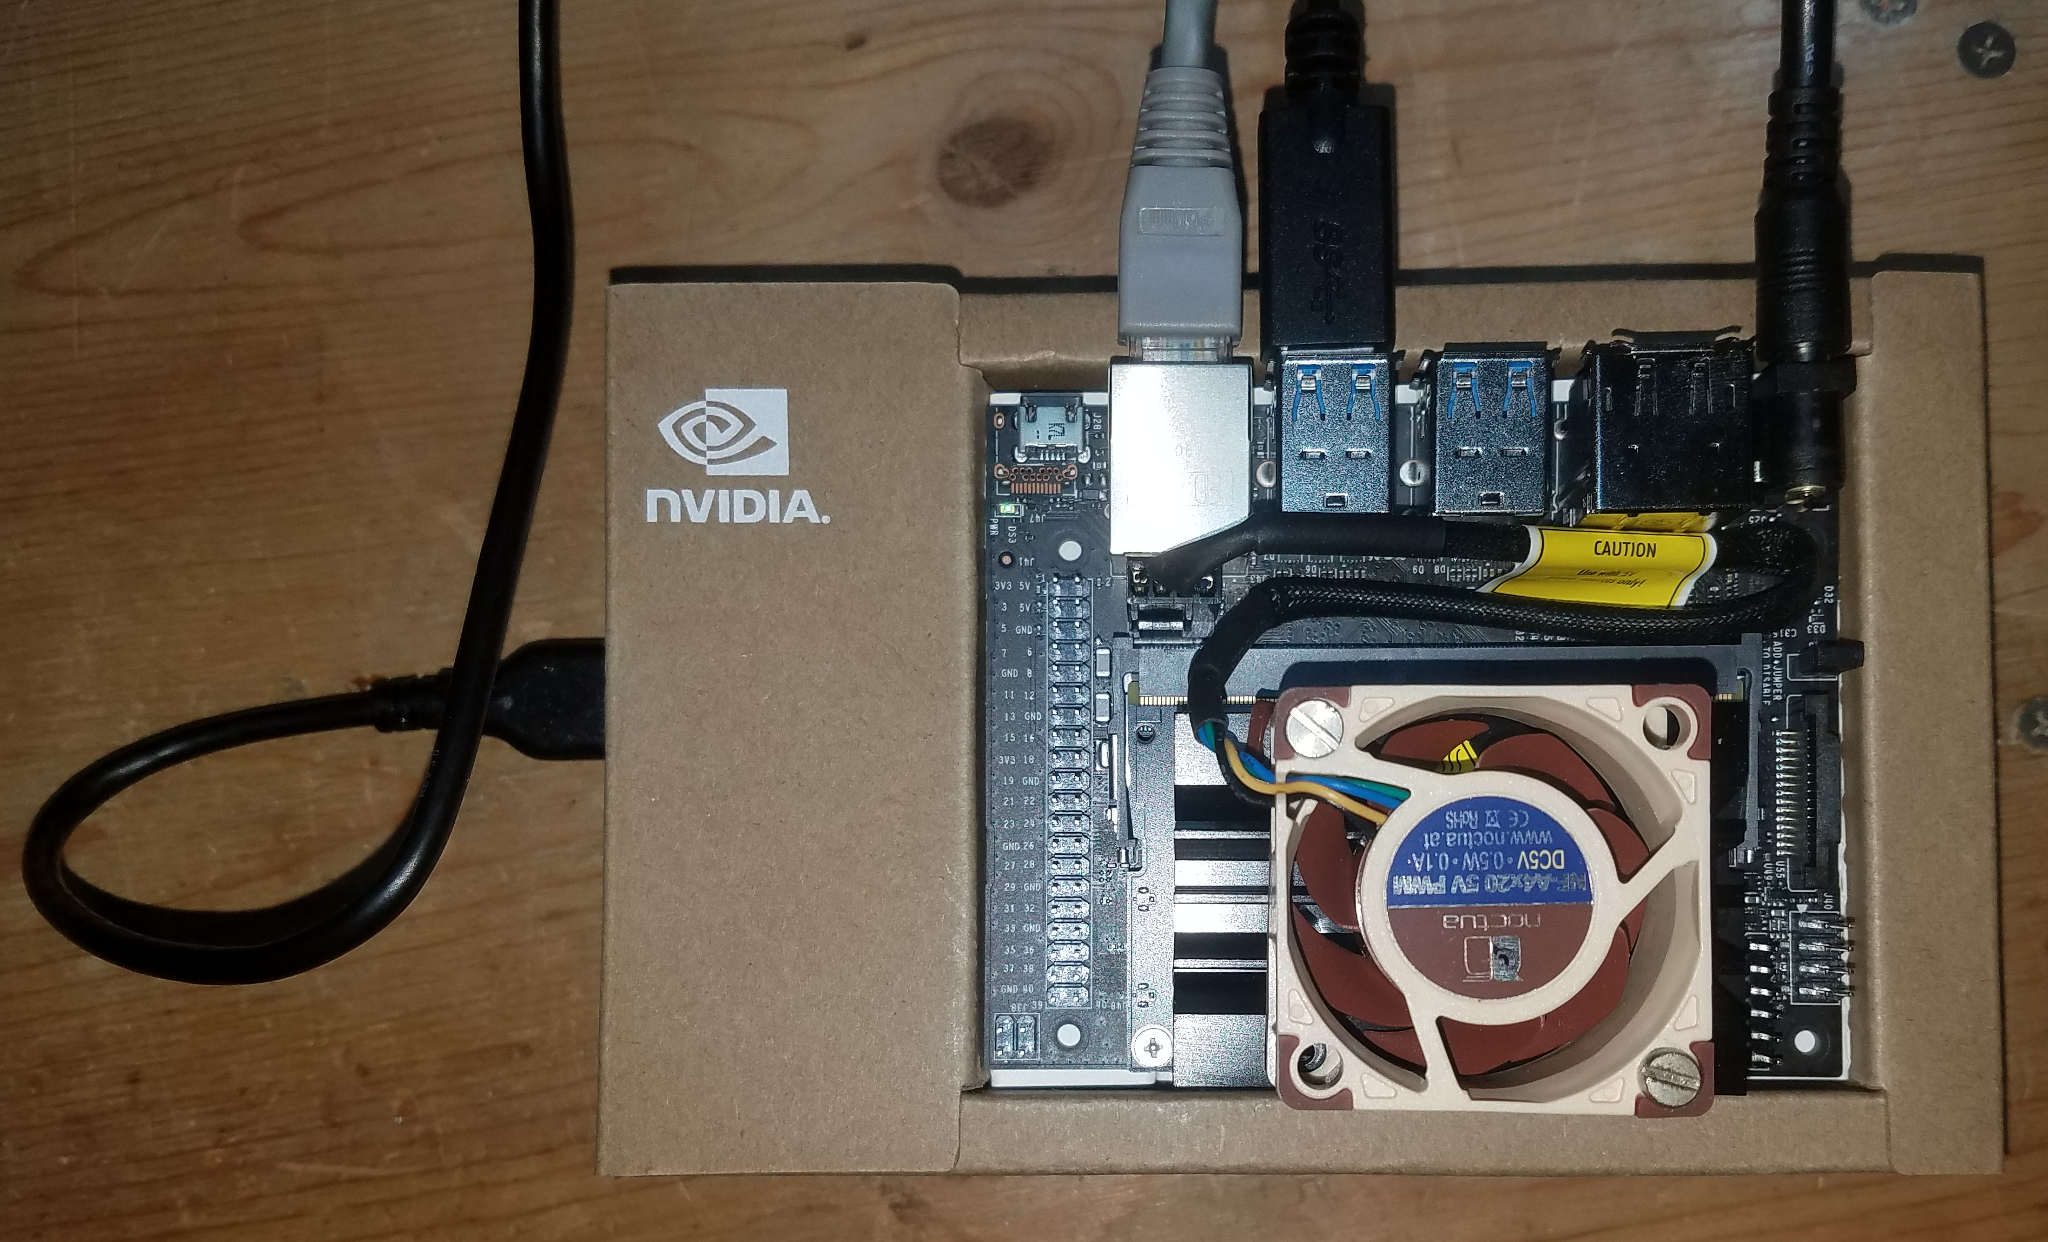
\includegraphics[width=100mm]{TopView.jpg}
\caption{Top view of the Jetson Nano placed in its box with fan mounted to the
heat sink and Ethernet, USB drive, and power connected.
\label{Fig:TopView}}
\end{figure}

First, the SD card image needs to be downloaded from NVIDIA's web page
\cite{JetsonNano19} and copied to a micro SD card.  This step is fairly
straightforward and works exactly as described on NVIDIA's web page.

The next thing one needs to do is to provide sufficient power to the board.  The
Jetson Nano has two pre-configured power modes, 5W and MAXN, and the kernel
image comes preconfigured for MAXN mode, which will let the unit draw about 4~A
versus the 1~A it will draw in 5W mode.  One can switch between the modes
via the command line tool \verb|nvpmodel|.  Note that the mentioned currents do
not include any power that USB peripherals or an optional fan might require and
that the USB~3 connectors are rated for up to 900~mA each---the power
requirements for the fan with only 100~mA are almost negligible in this context.
 When the board is powered via the micro-USB connector, however, it can only
draw up to 2~A over that connector. If that is not enough, and it will not be
enough for many applications and/or when peripherals are attached via the USB~3
ports, the Jetson Nano will simply shut down. Therefore, a jumper should be
installed at J48 (see Figure~\ref{Fig:J48}), and a sufficiently strong 5~V power
supply should be connected to the barrel jack.  We use a ALITOVE 5~V 15~A AC to
DC Power Supply for our experiments.

\begin{figure}[ht!]
\centering
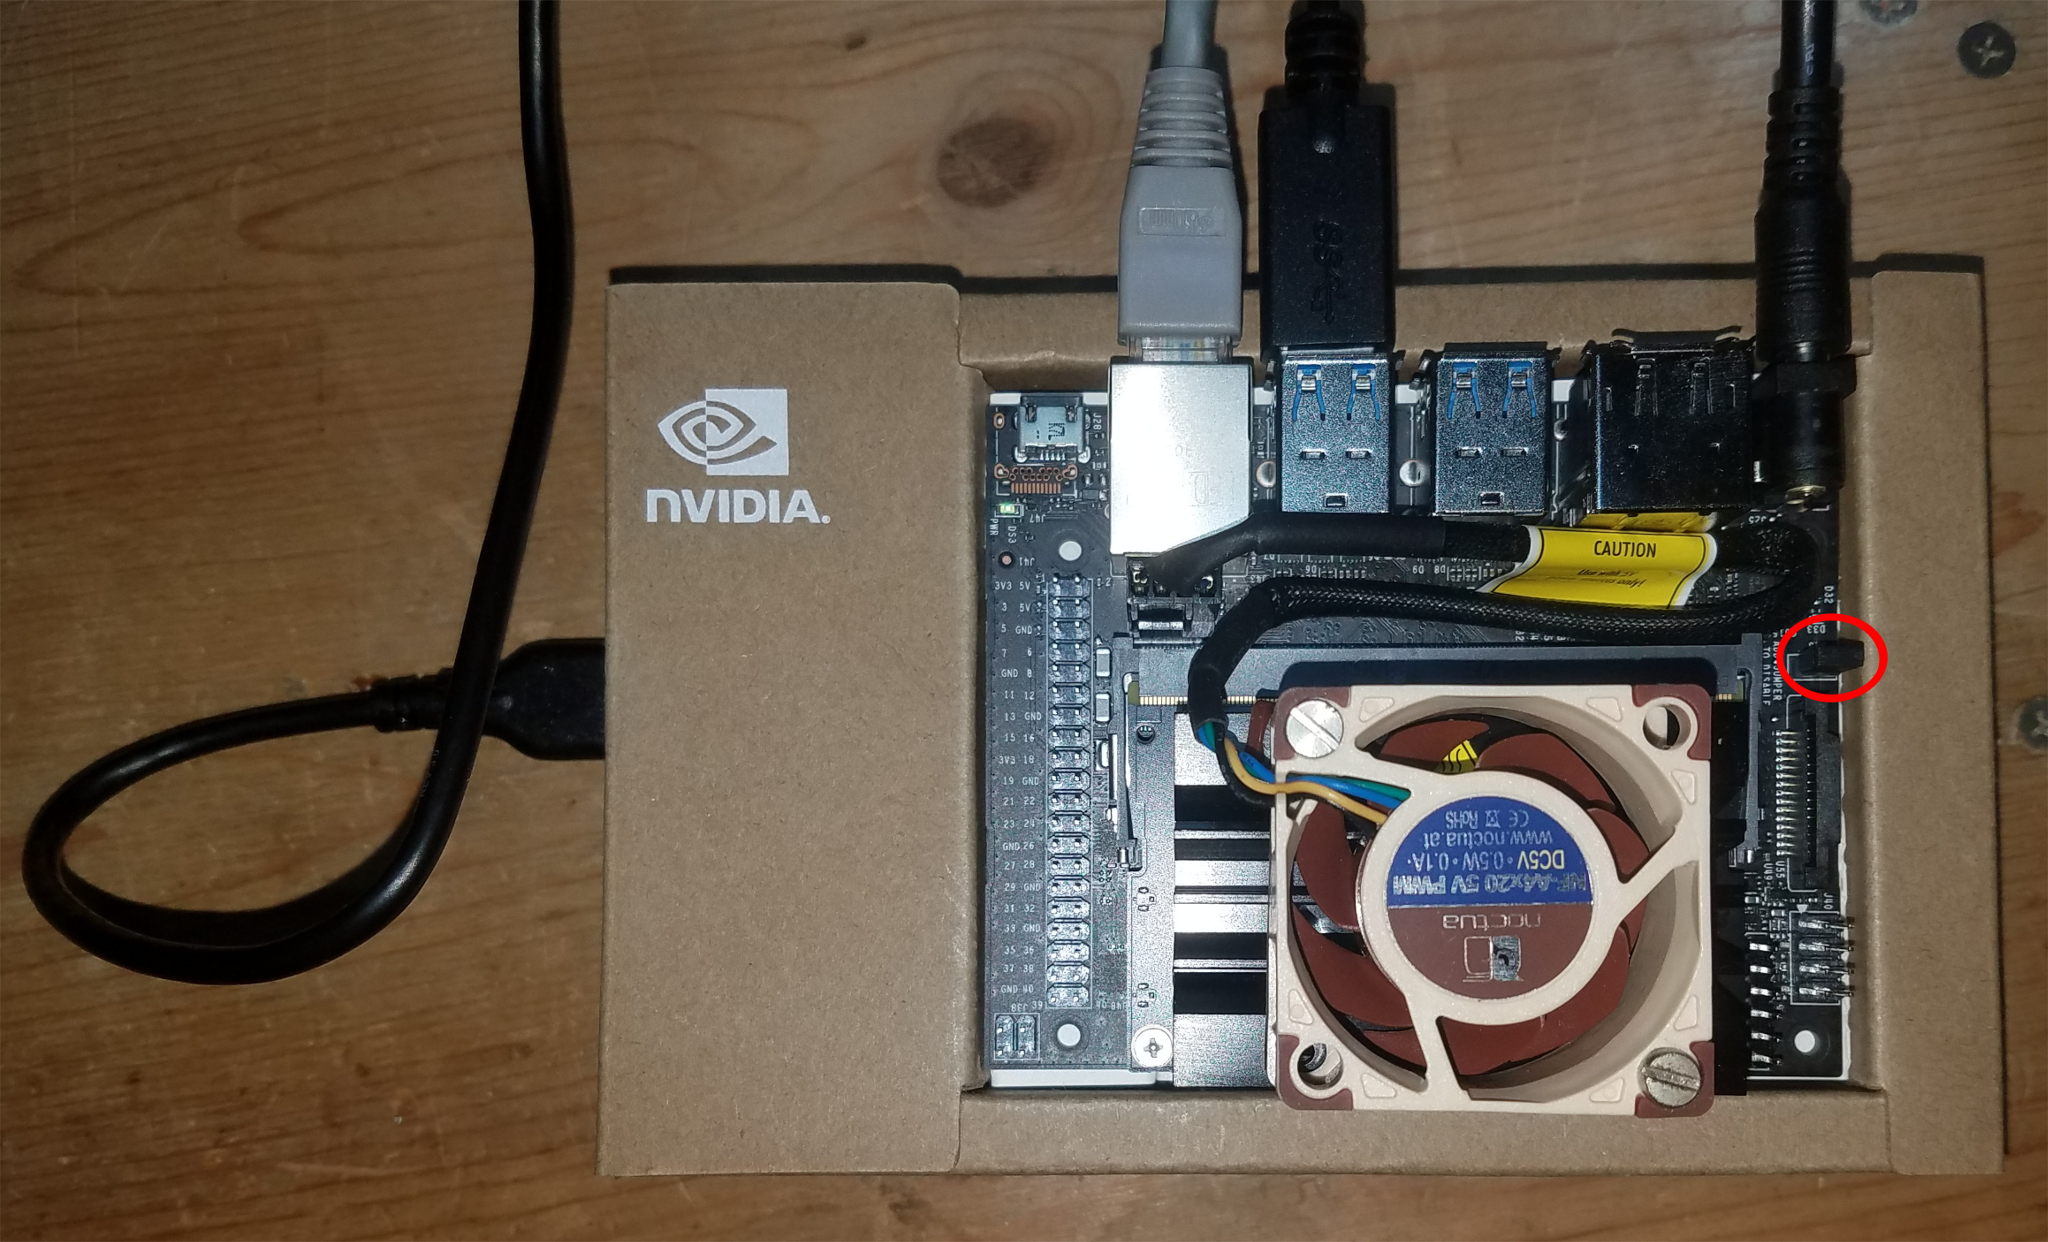
\includegraphics[width=80mm]{J48.jpg}
\caption{Jumper J48 placed on Jetson Nano Developer Kit board.
\label{Fig:J48}}
\end{figure}

Then, it may be a good idea to mount a 40~mm fan on top of the heat sink.  It
will draw a little extra power, but it will prevent the system from
down-clocking in heavy computational load situations.  We use the
NVIDIA-recommended Noctua NF-A4x20 5~V PWM, Premium Quiet Fan, which we
connected to the PWM connector that is provided for this purpose (see
Figure~\ref{Fig:PWM}).  One word of caution: the mounting holes in the heat
sink of the Jetson Nano are not threaded. Therefore, either self-tapping M3
screws are to be used, as suggested by NVIDIA, or the holes need to be tapped
before the fan can be installed with regular M3 machine screws.

\begin{figure}[ht!]
\centering
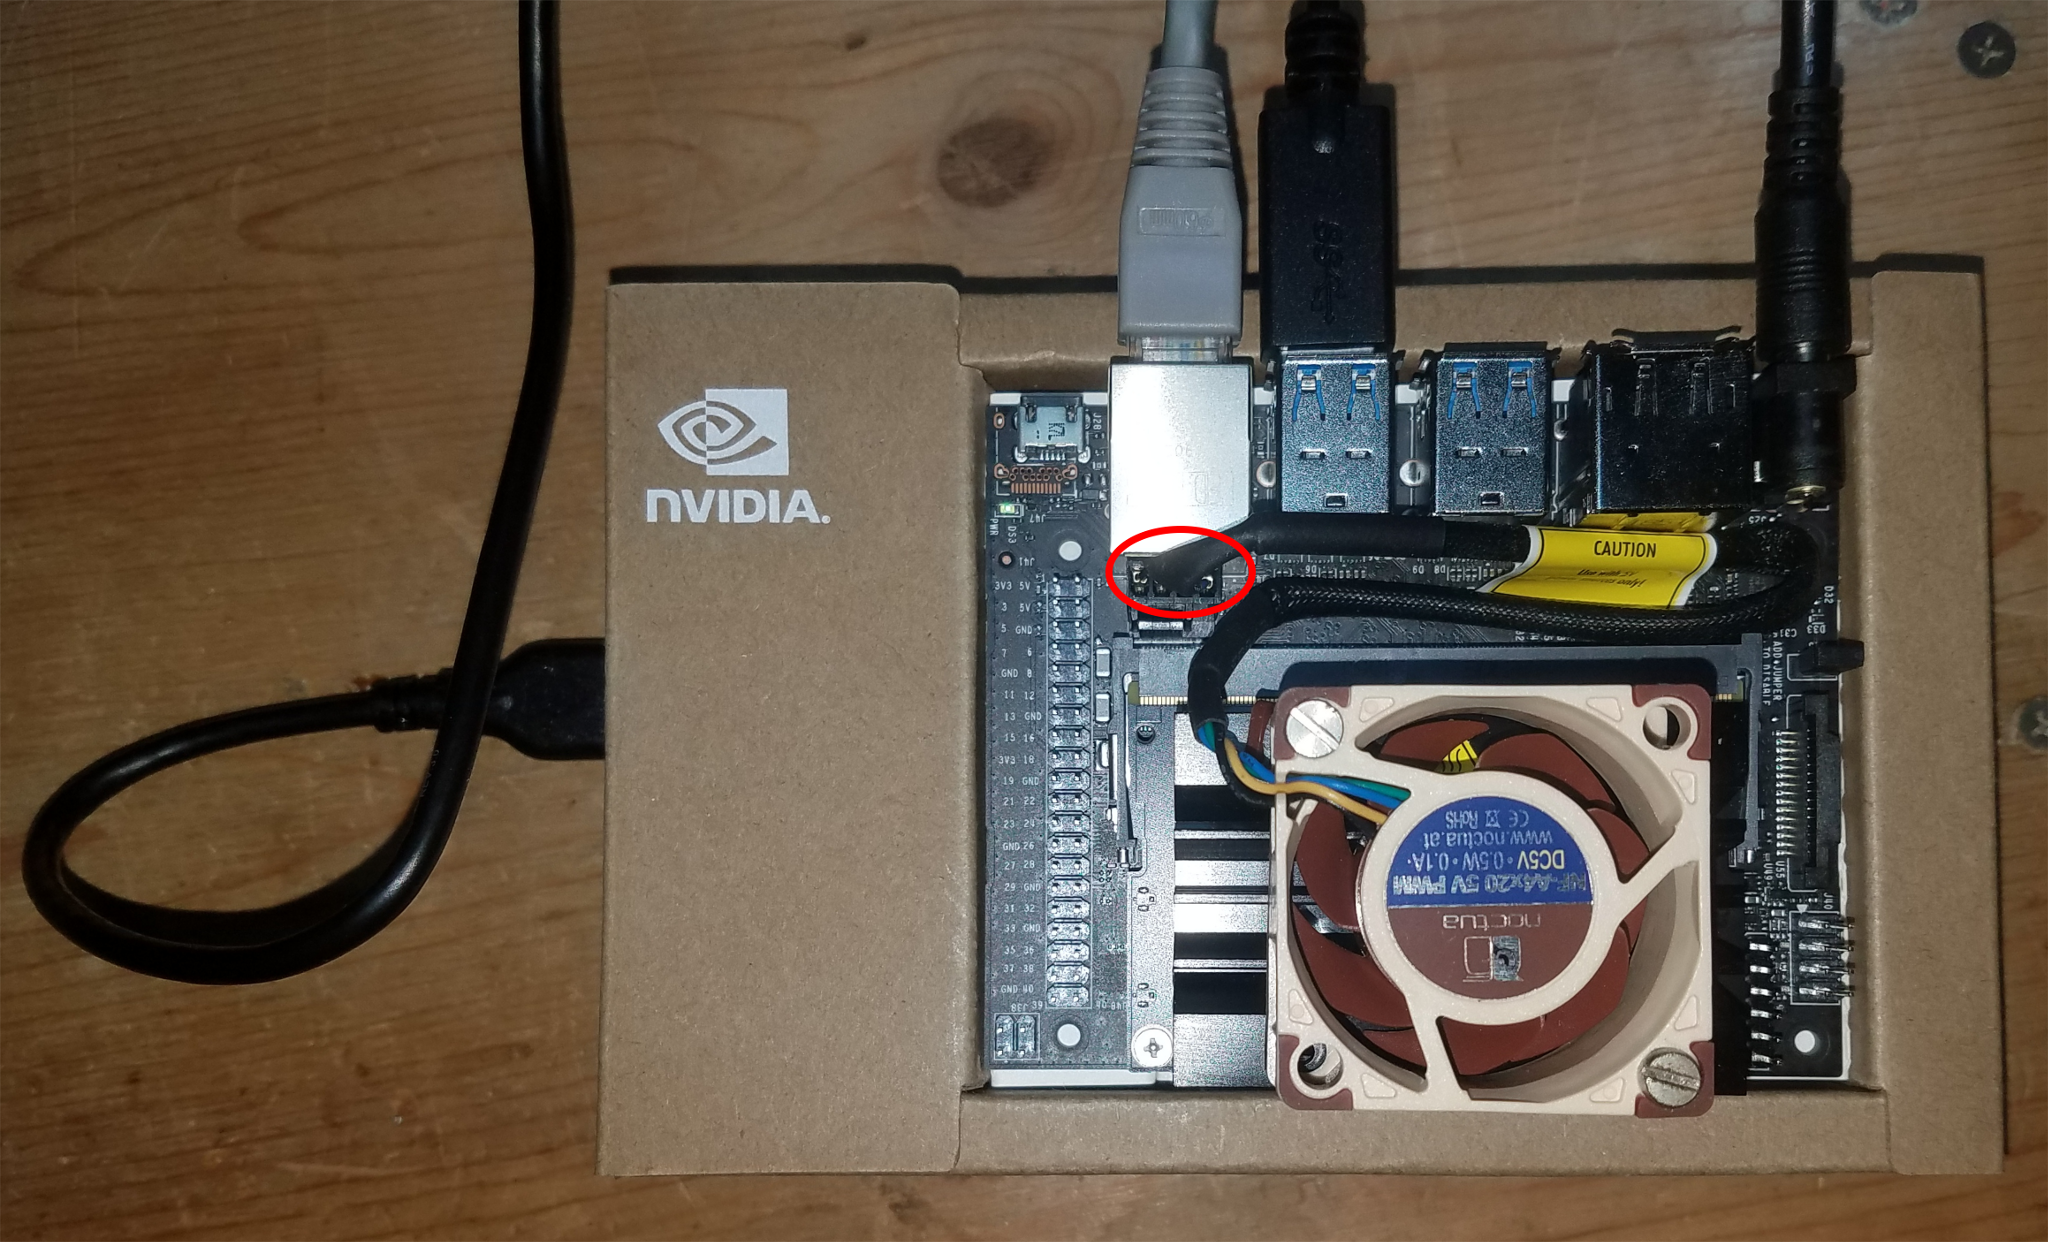
\includegraphics[width=80mm]{PWM.jpg}
\caption{Fan connected to the PWM connector.
\label{Fig:PWM}}
\end{figure}

Further, even though many people do just that, it is not advisable to run any
SoB, such as the Jetson Nano\footnote{Or the Raspberry Pi we used in the
experiments, for that matter.}, from a micro SD card.  These cards are much
slower than USB drives, and they are not designed for the frequent access
patterns associated with mass storage devices in Linux computers---they are
{\em not} SSD drives! Therefore, it is a good idea to use an external USB drive,
either mechanical or SSD, connected to the Jetson Nano. Unfortunately, the
kernel that was loaded onto the micro SD card does not support USB~3 drives.
Therefore, a different kernel source tree needs to be downloaded.  A good source
for that is \verb|JetsonHacksNano/rootonUSB| on github. This repository can be
cloned via git or just downloaded as a zip file.  It needs to be downloaded on
the micro SD card of the Jetson Nano and then compiled there.  This is made very
simple with a shell script that is packaged with the kernel source that can be
executed once we have navigated to the directory of the repository as
\begin{small}
\begin{verbatim}
 $ sudo ./buildKernel.sh
\end{verbatim}
\end{small}
This will place the kernel image in /boot/Image, which means that if the Jetson
Nano is rebooted, it will boot using that new kernel image.

Next we need to prepare the USB drive for use as a Linux disk.  In our case, we
have used an inexpensive mechanical 1~TB external USB drive, specifically the
Toshiba Canvio Basic with a 480~Mb/s data rate.  To keep the external USB drive
together with the Jetson Nano as a unit, we have cut a slot in its cardboard
box, big enough to accommodate the external USB drive (see
Figure~\ref{Fig:SideView}).

\begin{figure}[ht!]
\centering
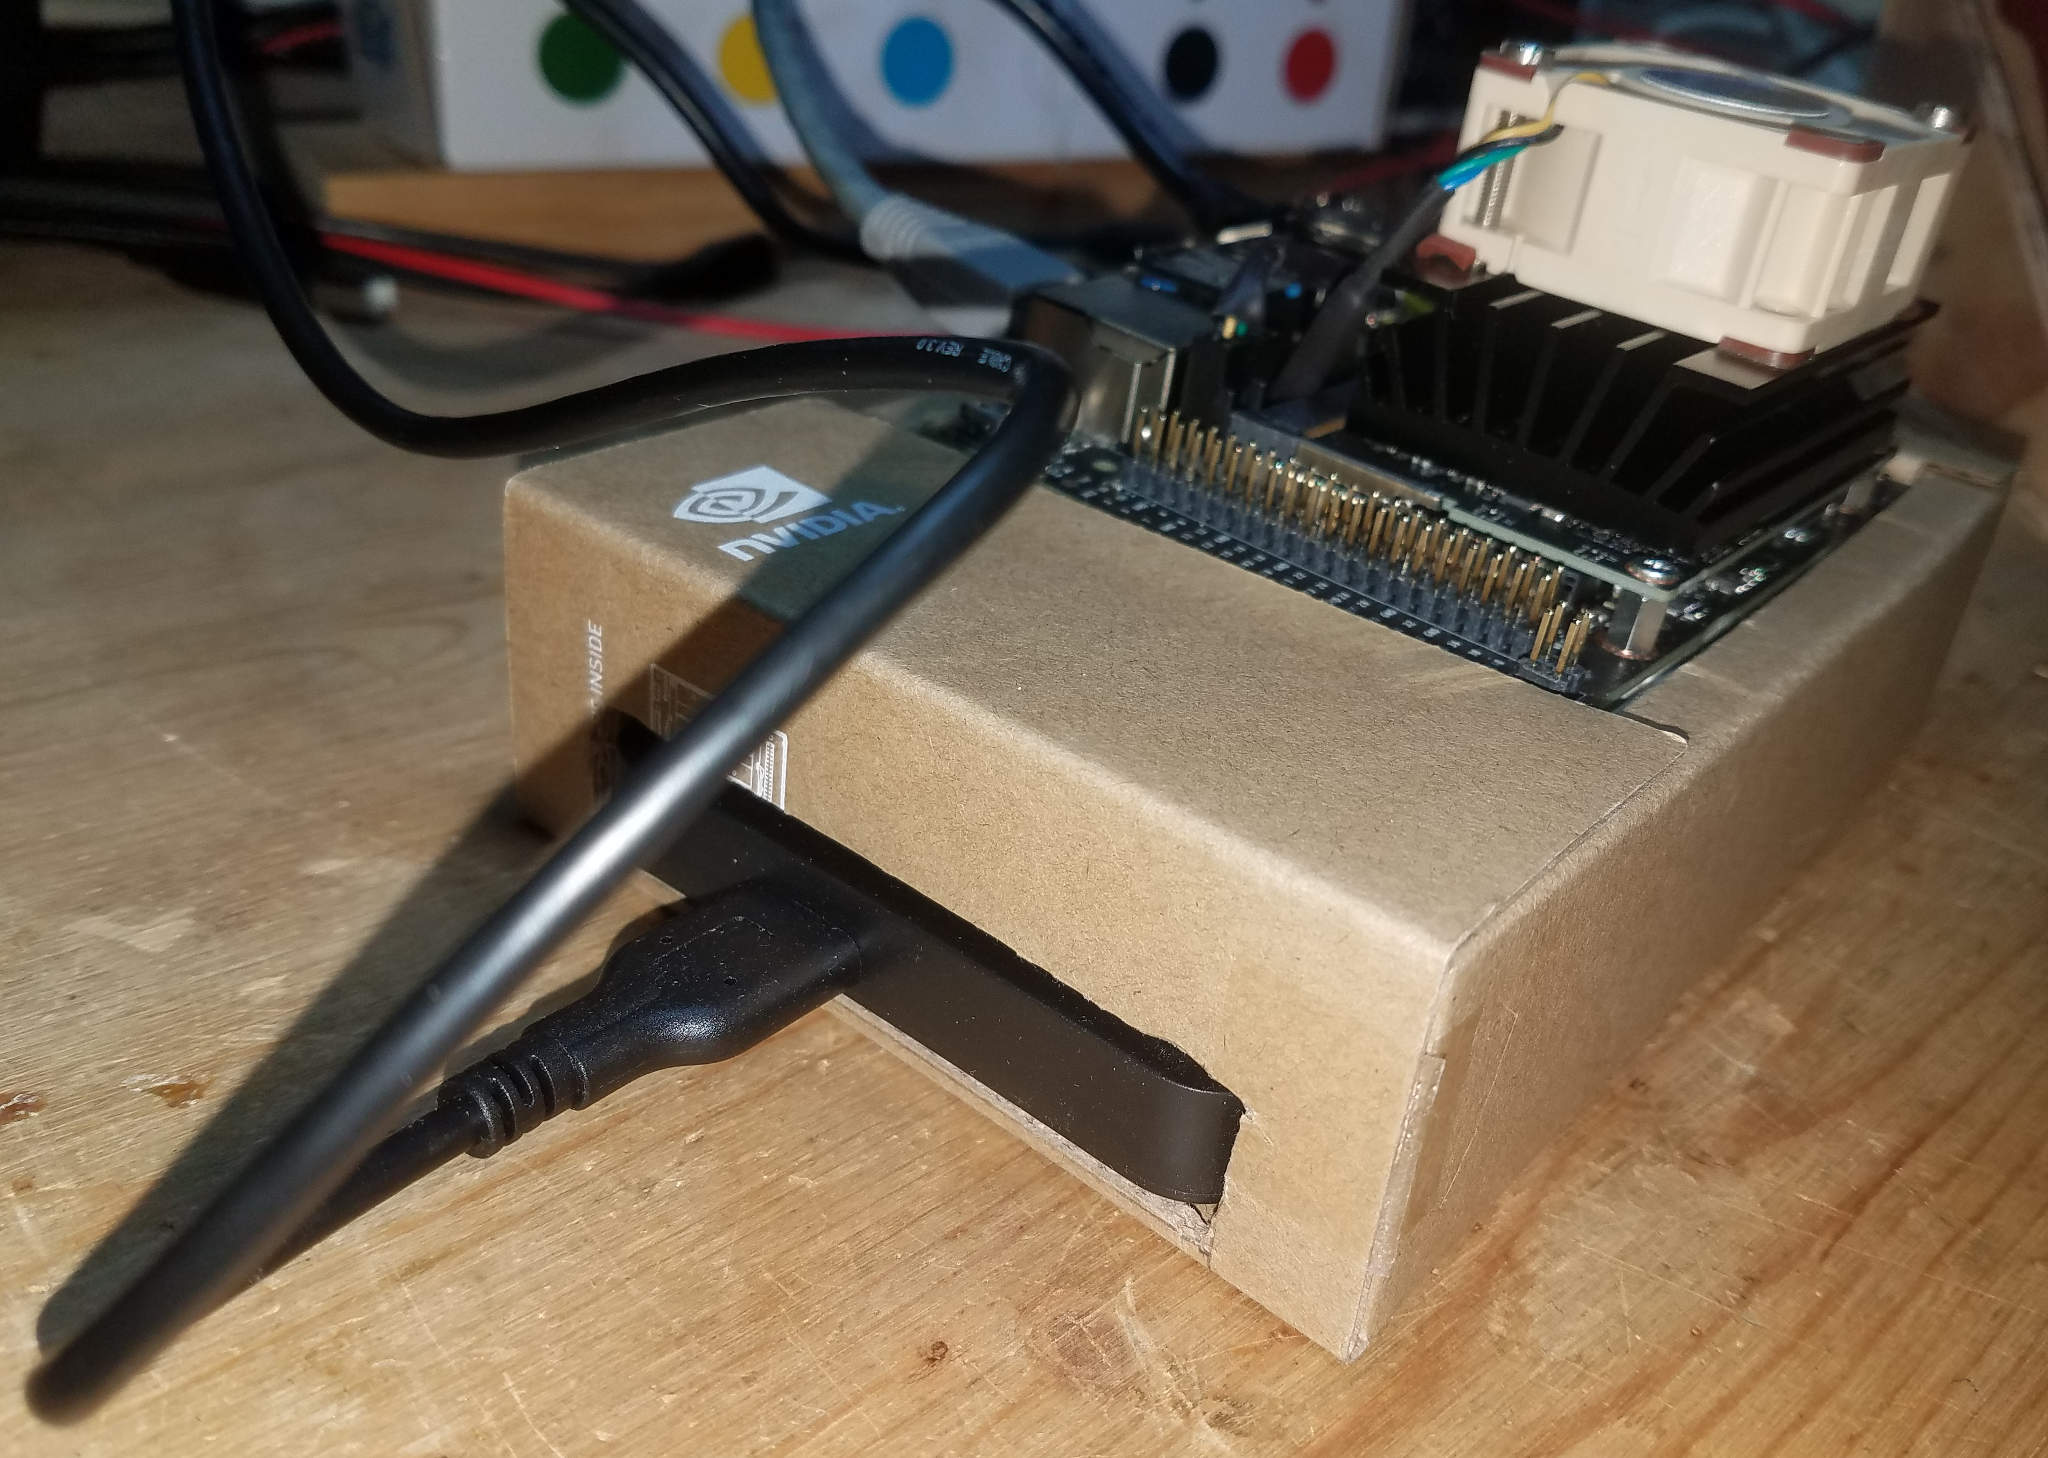
\includegraphics[width=80mm]{SideView.jpg}
\caption{Side view of the Jetson Nano box showing slot for external USB drive.
\label{Fig:SideView}}
\end{figure}

We will use \verb|gparted| to partition and format the USB drive, which
therefore also needs to be installed on the Jetson Nano (see
Section~\ref{sec:Software Setup}). We use about 64~GB for the root file system,
8~GB for swap space, and the rest of the disk space for \verb|/home| and format
the disk for the Ext4 file system.

Then the root file system needs to be copied over from the micro SD card to the
USB drive.  The \verb|rootonUSB| repository has a convenience script for that,
which we will use, supplying the volume name we gave to our USB drive in
\verb|gparted| as an argument
\begin{small}
\begin{verbatim}
 $ sudo ./copyRootToUSB.sh -v <volume name>
\end{verbatim}
\end{small}
Once the kernel is compiled and placed on the micro SD card as well as the USB
drive, we can ``pivot the root,'' i.e.\ tell the Jetson Nano to just use the
micro SD card as a bootloader and then switch to the USB drive.  We do this by
editing the file \verb|extlinux.conf| in \verb|/boot/extlinux| to look
something like this
\begin{small}
\begin{verbatim}
TIMEOUT 30
DEFAULT primary

MENU TITLE p3450-porg eMMC boot options

LABEL primary
      MENU LABEL primary kernel
      LINUX /boot/Image
      INITRD /boot/initrd
      APPEND ${cbootargs} rootfstype=ext4 root=/dev/sda1 rw rootwait

LABEL sdcard
      MENU LABEL primary kernel
      LINUX /boot/Image
      INITRD /boot/initrd
      APPEND ${cbootargs} rootfstype=ext4 root=/dev/mmcblk0p1 rw rootwait
\end{verbatim}
\end{small}
With these changes, the Jetson Nano should be using the USB drive as a
root file system after reboot.

For all benchmark applications that require access to files residing on the
local disk during training or test, we store all such files on the external
USB drive of the Jetson Nano and remotely mount this drive at the other systems
and access the data on it via the Gigabit LAN from the other systems. This is to
assure that the relatively slow disk does not unfairly disadvantage the Jetson
Nano. For all benchmark experiments, we run the Jetson Nano as a ``headless
server,'' i.e.\ without keyboard, mouse, or monitor and use \verb|xfreerdp| to
log into it from other systems on the LAN, which requires the installation of
\verb|xrdp| (including enabling it using \verb|systemctl|) on the Jetson Nano.

All Jetson Nano paraphernalia used in this study outside of standard cables,
screws and jumpers, which are considered standard lab stock, were sourced
through Amazon.com.



\subsection{Software Setup}
\label{sec:Software Setup}
Of course, there are many different application domains one can imagine to
showcase a dedicated GPU, amongst which graphics intense applications and
visualizations certainly play a dominant role, and the software packaged with
the Jetson Nano installation kernel contains several interesting graphical
applications for that purpose.  However, our focus is on the AI application
niche that was targeted by NVIDIA for the Jetson Nano and its GPU, and the AI
applications that stress the capabilities of any compute engine the furthest are
certainly Deep Learning applications \cite{Goodfellow16}, \cite{Raschka16}.
That's why we focus on Deep Learning applications for this study exclusively.

The Deep Learning community has widely embraced Python with Jupyter notebooks as
a working environment for online experimentation, in part because with that
environment it makes no difference whether one is working in the cloud or
locally.  In that working environment, the Python package Keras is our tool of
choice for Deep Learning experiments, mostly because of its ease of use.  Keras
works with several backends, TensorFlow, Theano, and CNTK, from which we
selected TensorFlow as our backend of choice. TenesorFlow, in turn, uses several
compute engine backends for standard numerical tasks, such as BLAS and LAPACK
for computations that are performed on the regular CPU(s), as well as CUDA and
cuDNN to unleash the power of GPUs to accelerate its most compute intensive
tasks in cases where the system is equipped with appropriate GPUs.

To prepare for the experiments, some additional Python packages need to be
installed on top of a regular Python~3 environment, which should probably
include Jupyter, and, of course, pip.  However, especially on the Jetson Nano,
chances are that packages need to be built and therefore, the Unix build tools
need to be installed in case they are not already present.  All packages from
distros on the Jetson Nano are downloaded using
\begin{verbatim}
 $ sudo apt install <package name>
\end{verbatim}
The build packages we get from the distro are
\begin{itemize}[noitemsep]
  \item build-essential
  \item cmake
  \item unzip
  \item pkg-config
\end{itemize}

In addition, as mentioned above, we need the numeric libraries BLAS and LAPACK
also from distro
\begin{itemize}[noitemsep]
  \item libopenblas-dev
  \item liblapack-dev
\end{itemize}

Then we need to start installing Python packages specifically needed for Deep
Learning.  We strongly recommend to choose the packages from the particular
distros wherever they are available over the generic Python packages.  The
Python packages we prefer to get from our distro are
\begin{itemize}[noitemsep]
  \item python3-setuptools
  \item python3-all-dev
  \item python3-numpy
  \item python3-scipy
  \item python3-matplotlib
  \item python3-libyaml-dev
  \item python3-cpuinfo
  \item python3-psutil
\end{itemize}
The last two packages are only needed to list system information in the log
files.

Where Python packages cannot be obtained from distro, which, at the time of
writing, is still often the case on the Jetson Nano, they need to be installed
via pip, i.e.\
\begin{verbatim}
 $ sudo pip3 -H install <package name>
\end{verbatim}
obviously here the package names don't use the ``python3-'' prefix\footnote{We
use Python~3 exclusively---never Python~2.}.  On the Jetson Nano, pip will often
need to compile the sources to build the packages, which may take a while.

Next, on the Jetson Nano and all machines with GPU support, we also need
CUDA, and, optionally, cuDNN.  Then we need to install TensorFlow, and, finally,
Keras.  We start with the packages that we only need where GPUs are present; on
benchmark contenders without GPU, as is the case in our study in all systems
outside of the Jetson Nano, we can skip the installation of CUDA and cuDNN. On
the Jetson Nano, CUDA~10.0 comes pre-installed, but cuDNN was not available for
this architecture at the time of writing. For instructions how to install CUDA
and cuDNN on any other system with GPU support, we refer to the steps outlined
in \cite{Chollet18}, which are very easy to follow.

Now it is time to install TensorFlow.  Which package exactly to install depends
on whether or not the system it is to be installed on has GPU support or not.
Either way, TensorFlow needs to be installed via pip, and the package name is
either tensorflow or tensorflow-gpu, depending on whether or not GPU support is
available.

We hit one minor roadblock when we installed TensorFlow on Gandalf, however.
The old AMD Phenom has no AVX or SSE~4.2 instructions, which TensorFlow versions
later than 1.5 requires.  This forced us to roll back to TensorFlow version
1.5.0 on Gandalf only.

Lastly, we need to install Keras.  This is very straightforward, as it should
be installed directly with pip, and it installed without any problems on all of
our systems.

\subsection{The Benchmark Applications}
\label{sec:The Benchmark Applications}
We take all of our applications straight out of Chollet's book \cite{Chollet18}.
To facilitate experimentation, we wrote a small wrapper that calls the
individual benchmark applications and logs their results in a log file that
identifies not only the name of the application but also the parameters of the
system that executed the application, such that the results are easily
attributed to the system they were achieved with.

Table~\ref{tab:Tasks} shows the training and test samples sizes as well as the
epochs and batch sizes used for the experiments.  Table~\ref{tab:Architectures}
shows the net architectures used for the same experiments.  They are all the
same as in \cite{Chollet18}.

\begin{table}[ht!]
\begin{center}
\begin{small}
\begin{tabular}{|l|r|r|r|r|} \hline
                  & Train. Samp. & Test Samp. & Epochs & Batch Size \\
                  \hline \hline
MNIST Digits 1D   &  60000 &  10000 &  5 & 128 \\ \hline
IMDB              &  25000 &  25000 &  4 & 512 \\ \hline
Reuters           &   8982 &   2246 &  9 & 512 \\ \hline
MNIST Digits 2D   &  60000 &  10000 &  5 &  64 \\ \hline
Dogs vs Cats      &   2000 &   1000 & 15 &  20 \\ \hline
IMDB Embedded     &  25000 &  25000 & 10 &  32 \\ \hline
MPI Weather       & 200000 & 120406 & 10 & 128 \\ \hline
MPI Weather Conv. & 200001 & 120407 & 10 & 128 \\ \hline
\end{tabular}
\end{small}
\caption{Benchmark tasks parameters.}
\label{tab:Tasks}
\end{center}
\end{table}

\begin{table}[ht!]
\begin{center}
\begin{small}
\begin{tabular}{|l|r|r|r|} \hline
                  & Input Shape & Net Architecture & Parameters \\
                  \hline \hline
MNIST Digits 1D   &  (784,)        &  (512, 10)    & 407050 \\ \hline
IMDB              &  (10000,)      &  (16, 16, 1)  & 160305 \\ \hline
Reuters           &  (10000,)      &  (64, 64, 46) & 647214 \\ \hline
MNIST Digits 2D   &  (28, 28, 1)   & ((26,26,32), (11,11,64), (3,3,64), 64, 10)
                                                               &  93322 \\
\hline
Dogs vs Cats      & (150, 150, 3) & ((148,148,32), (72,72,64), (34,34,128),
                                                                   & 3453121 \\
                  &                & (15,15,128), (7,7,128), 512, 1)
                                                            &  \\ \hline
IMDB Embedded     &  (50,) &  ((50,8), 400, 1) & 80401 \\ \hline
MPI Weather       & (21,) & (32, 1) & 5217 \\ \hline
MPI Weather Conv. & (21,) & (32, 32, 32, 1) & 14817 \\ \hline
\end{tabular}
\end{small}
\caption{Benchmark tasks network architectures.}
\label{tab:Architectures}
\end{center}
\end{table}

In the following, we will give only a very brief description of the different
experiments.  Since teaching the idiosyncrasies of Deep Learning methods,
especially for more than one-dimensional datasets is beyond the scope of this
report, we refer the reader interested in any more details to \cite{Chollet18}
for the particular experiments and to \cite{Goodfellow16} for a more in-depth
coverage of Deep Learning networks.

\subsubsection{MNIST Digits 1D}
\label{sec:MNIST Digits 1D}
This experiment uses a set of 70,000 images of handwritten digits, each stored
as a 28 by 28 pixels gray-value image.  The dataset comes pre-packaged with
Keras and is split into 60,000 images as training set and 10,000 images as test
set.  The images have originally been assembled by NIST but have later been
modified to better mix the sources of the digits in training and test set; they
were also normalized in size and gray level intensity (hence the ``M'' in
MNIST).  In this experiment the pixels of the images are re-arranged to form
simple vectors for a very easy one-dimensional Deep Learning experiment.

Here we use a net with only one hidden layer with 512 nodes and an output layer
with (obviously) 10 nodes, one for each category.  We train with 5 epochs and a
batch size of 128.

\subsubsection{IMDB}
\label{sec:IMDB}
Here we use 50,000 highly polarized reviews of movies from the Internet Movie
DataBase which we want to classify into positive and negative reviews. Again,
the data comes pre-packaged with Keras and is split into 25,000 training and
25,000 test samples with the same number of positive and negative reviews in
each set.  To make these texts palatable for neural networks, they need to be
converted into vectors of real numbers.  To do this, the texts are first
converted into lists of integers where each integer represents a particular word
but where we use only the 10,000 most frequently occurring words in the
texts---the others simply don't encode at all.  Then, following
\cite{Chollet18}, we engage in a rather wasteful encoding scheme that also
eliminates the information stemming from the word sequence whereby we assign to
each review a 10,000-dimensional vector that contains all zeros except for the
positions that correspond to a word that is contained in the given review; at
those positions they contain a one, even if the word occurred more than once.

We us a net with two hidden layers with 16 nodes each, and since this is a
binary classification task only one node in the output layer.  We train with 4
epochs and a batch size of 512.

\subsubsection{Reuters}
\label{sec:Reuters}
In this experiment we use a database of 11,228 newswire reports from Reuters
with wires pertaining to 46 different categories of news.  This dataset too
comes with Keras and is split into 8982 training samples and 2246 test
samples.  To convert the text into vectors of real numbers, we use the same
method as described in Section~\ref{sec:IMDB}.

We train a net with two hidden layers with 64 nodes each and use one node for
each of the 46 categories in the output layer.  We train with 9 epochs and a
batch size of 512.

\subsubsection{MNIST Digits 2D}
\label{sec:MNIST Digits 2D}
In this experiment we use the same dataset as described in
Section~\ref{sec:MNIST Digits 1D}.  However, this time we we will feed the
images as two-dimensional images directly to the net and will not convert them
into one-dimensional vectors first.  To allow that, we will use what is called a
convnet, i.e.\ a neural network that acts like a convolution kernel in image
processing.  Our convnet will start out with a 3 by 3 convolution kernel
producing 32 ``features'' as the first hidden layer, still arranged in a
two-dimensional pattern.  We will then reduce the size of each of the 32 feature
matrices by a 2 by 2 maximum non-linear filter, leaving us with 32 feature
matrices of size 13 by 13\footnote{The convnet reduces the image size already as
data points at the borders are not defined.}. Then, in the next hidden layer, we
apply another convnet using a 3 by 3 window, this time producing 64 features.
Again, we will reduce the size with a 2 by 2 maximum non-linear filter and apply
yet another hidden convnet layer, producing 64 features with 3 by 3 kernels.  We
will finally ``flatten'' the ``feature images'' to regular vectors, apply a
final hidden layer with 64 nodes feeding into the output layer with 10 nodes for
the 10 categories of the digits.

We train with 5 epochs and a batch size of 64.

\subsubsection{Dogs vs Cats}
\label{sec:Dogs vs Cats}
Here again we use datasets of images, in this case even three-dimensional images
since they are color images.  This dataset did not come with Keras and had to
be downloaded from Kaggle (\verb|www.kaggle.com/c/dogs-vs-cats/data|).  The full
dataset contains 25,000 images of dogs and cats of which we randomly selected
2,000 images for training and 1,000 images for testing to reduce the problem
size and hence the computation time to a more manageable level and since we
were not interested in achieving the best possible classification result but
rather in performance differences of different systems.  We also instructed
Keras to reshape all images to 150 by 150 pixels.

For the net architecture we chose again convnets as in Section~\ref{sec:MNIST
Digits 2D} which we interspersed with 2 by 2 maximum filters.  All in all, we
used 5 hidden layers reducing the image or ``feature map'' size from 148 by 148
to 7 by 7 in four steps, but, at the same time, increasing the number of
features from 32 to 128 and finally to 512.  Since this again is a binary
classification task, the output layer has only one node.

We train with 15 epochs and a batch size of 20.

\subsubsection{IMDB Embedded}
\label{sec:IMDB Embedded}
This experiment uses the same dataset of movie reviews as described in
Section~\ref{sec:IMDB}.  However, this time we use a word embedding scheme to
encode the text into vectors of real numbers instead of a single vector
with certain elements ``switched on.''  This has the advantage of being overall
less wasteful than what we have seen in Sections~\ref{sec:IMDB} and
\ref{sec:Reuters} even though it comes at the expense of an additional dimension
for the embedding vector. In other words, at each training step, the subsequent
layer will be presented with a number of embedding vectors that equals however
many words in the text we want to look at, which in our case is only the first
50 words. Word embedding is done at the expense of higher computational effort
when compared to Section~\ref{sec:IMDB}, since this mapping will be part of what
is learned from the training set and not programmed {\sl a priori}.

In total our net consists only of the hidden embedding layer, embedding every
text integer into an 8-dimensional vector and an output layer with a single
node.  We train with 10 epochs and a batch size of 32.

\subsubsection{MPI Weather}
\label{sec:MPI Weather}
This dataset was downloaded from the Max Planck Institute for Biogeochemistry
in Jena, Germany.  We downloaded their weather data from 2009 to 2016 and tried
to predict next days temperature from all the 21 weather-relevant measurements
they collected every ten minutes over the last 5 days.  Since this is a
regression task and not a classification task, we have no classification
accuracy to report.  Since we are dealing with time series, we use a recurrent
neural network (RNN) for this task to acknowledge the fact that successive
measurement vectors are not independent of each other and that there is valuable
information in the numerical progression from one measurement vector to the
subsequent ones.  We will sub-sample the data every 6th step thus dealing with
only one measurement vector per hour.  For the prediction of the temperature 24
hours ahead, we will use the data from the last 5 days or 720 total observation
vectors.  Therefore, for each training step, we will present the data of five
days worth of measurements as measurement vector and the data 24 hours from
``now'' as the target.  We use a Gated Recurring Unit (GRU) with 32 nodes as
first hidden layer and a single node output layer for the regression task.

We train with 10 epochs and a batch size of 128.


\subsubsection{MPI Weather Convnet}
\label{sec:MPI Weather Conv.}
This last experiment uses the same dataset of weather data as described in
Section~\ref{sec:MPI Weather}.  However, we now also apply the concept of
convnets, albeit this time one-dimensional ones, not the two-dimensional ones
we used for images.  We use two hidden one-dimensional convolution layers with
5 taps each, both producing 32 ``features'' with one non-linear maximum finding
unit with 3 taps between them.  We then use the same GRU layer as described in
Section~\ref{sec:MPI Weather}, followed by a single node output layer.

Again, we train with 10 epochs and a batch size of 128.



\section{Experimental Results}
\label{sec:Experimental Results}
Here we will present the results of the benchmark experiments outlined in
Section~\ref{sec:The Benchmark Applications}.  Without considering Boromir,
what we would expect is a superior performance of Gandalf and Bilbo, based on
the number of cores, processor speed and bit-depth of the architecture.  Frodo
would come in last with a shallow 32-bit architecture, a slow clock speed of
1.2~GHz, and it may not even succeed at all experiments with its measly 1 GB of
RAM (see Table~\ref{tab:Systems}).  The big unknown, obviously, is Boromir.
Without its GPU, it would be expected to rank somewhere between Frodo and Bilbo
or Gandalf.  But, as mentioned, that is without its GPU.  The big question is
how much of a performance boost we can expect from Boromir's GPU, and if we do
see such a performance increase, in which application areas will they be most
prominent.

To gain a comprehensive and yet compact representation of the experimental
results, we have collected them in three different tables, one to show the time
it took to train the (for all systems identical) net architectures, one to show
the time it took to execute the test set, and one where we listed the
classification accuracy on the test set for all systems.  We included this
last table to see whether the reduced bit depth of the floating point numbers
we used on Boromir impacted the accuracy of the results.  All numbers were
obtained by running each experiment five times and then taking the median of
those five values.  We chose the median over the average because Linux is not a
real-time operating system and we would expect some outliers when the CPU was
occupied doing some system tasks (which we did in fact observe).

First, Table~\ref{tab:Training Times} shows the training times for all the
eight different experiments on the four different computer systems.  There is no
entry for the IMDB experiment run on Frodo as it ran out of memory on this
experiment.

\begin{table}[ht!]
\begin{center}
\begin{small}
\begin{tabular}{|l|r|r|r|r|} \hline
                  &\multicolumn{4}{c|}{Training Time [s]} \\
                  & Gandalf &  Bilbo &  Frodo  & Boromir \\ \hline \hline
MNIST Digits 1D   &    33.7 &   29.3 &   255.8 &    63.2 \\ \hline
IMDB              &     5.9 &    8.1 &       - &    24.9 \\ \hline
Reuters           &     8.9 &    9.7 &    85.4 &    21.1 \\ \hline
MNIST Digits 2D   &   250.8 &  293.0 &  2378.1 &   263.5 \\ \hline
Dogs vs Cats      &  1463.5 & 2147.9 & 15105.3 &   550.2 \\ \hline
IMDB Embedded     &    29.3 &   29.6 &   118.3 &   125.4 \\ \hline
MPI Weather       &  1154.8 &  901.2 &  6634.0 &  6570.4 \\ \hline
MPI Weather Conv. &   730.5 &  622.7 &  4593.8 &  3027.8 \\ \hline
\end{tabular}
\end{small}
\caption{Training times.}
\label{tab:Training Times}
\end{center}
\end{table}

The first experiment with handwritten characters treated as one-dimensional
vectors shows the expected result without any noticeable boost from Boromir's
GPU.  The same is true for the experiment with the classification of IMDB movie
reviews and the Reuter news wires.

The first small surprise might be the classification of the MNIST database when
we treat the images of the handwritten characters no longer as one-dimensional
vectors but as two-dimensional images.  The performance of Frodo is, as
expected, very poor compared to that of Gandalf or Bilbo, but in this case,
Boromir's performance is very comparable to that of the thus far leading
contenders Gandalf and Bilbo and, in fact, beats Bilbo.

The biggest surprise by far, however, stems from the ``dogs vs cats''
experiment.  First, it appears as if Gandalf could, for the first time, take
advantage of its 6 cores over the 4 cores of Bilbo\footnote{We did notice
good use of all available cores while running the experiments.}.  The
performance ratio of Gandalf vs Bilbo is roughly that of 6 vs 4 cores directly.
The performance of Frodo is poor for this huge experiment, as expected for such
a small system. However, based on what we have seen so far, the performance of
Boromir must be called jaw dropping! 550.2~s vs 1463.5~s on Gandalf!  That is
almost a factor of three of performance improvement over the much bigger system
Gandalf and about a factor of 4 improvement over Bilbo, which we consider quite
remarkable.

The results of the experiment with the embedding layer to tackle the Internet
Movie Database classification task is, at the other hand, also surprising, just
in the opposite direction.  The performance of Boromir is right in the area
of Frodo, indicating that Boromir could not take any advantage of its GPU at
all for this experiment.

The results of the experiments using the MPI weather time series is no different
from the IMDB experiment with the embedding layer.  The performances of Frodo
and Boromir are virtually identical with a slight advantage for Boromir only
when using the convnet, but still more than three times worse than Gandalf.

Next we will have a look at the times it took to run the test sets as outlined
in Table~\ref{tab:Test Times}

\begin{table}[ht!]
\begin{center}
\begin{small}
\begin{tabular}{|l|r|r|r|r|} \hline
                  &\multicolumn{4}{c|}{Test Time [s]} \\
                  & Gandalf & Bilbo &  Frodo & Boromir \\ \hline \hline
MNIST Digits 1D   &     0.8 &   0.7 &    7.1 &     1.7 \\ \hline
IMDB              &     3.3 &   2.1 &      - &     8.0 \\ \hline
Reuters           &     0.8 &   0.3 &    1.6 &     0.8 \\ \hline
MNIST Digits 2D   &     3.8 &   3.1 &   26.8 &     5.8 \\ \hline
Dogs vs Cats      &    19.9 &  64.2 &  165.6 &    23.9 \\ \hline
IMDB Embedded     &     1.1 &   0.8 &    2.9 &     3.9 \\ \hline
MPI Weather       &    54.8 &  47.0 &  374.3 &   331.6 \\ \hline
MPI Weather Conv. &    37.8 &  38.8 &  319.4 &   134.4 \\ \hline
\end{tabular}
\end{small}
\caption{Test times.}
\label{tab:Test Times}
\end{center}
\end{table}

After having seen the results in Table~\ref{tab:Training Times}, these results
come as no big surprise.  The performance improvement of Boromir's GPU over
the other contenders in the ``Dogs vs Cats'' experiment is not  as pronounced as
it was during training, and ``only'' a little more than a factor of 2 better
than Bilbo and even worse than Gandalf, where again Gandalf is showing a
benefit from its larger number of cores over Bilbo.  The other results are in
the range where we would have expected them to be.

Lastly, we consult Table~\ref{tab:Test Accuracy} to see if the reduced bit
depth of Boromir's floating point number scheme has any negative impact on the
classification accuracy.  We note that the experiments using the MPI weather
data show no classification accuracy as they were no classification tasks.
\begin{table}[ht!]
\begin{center}
\begin{small}
\begin{tabular}{|l|r|r|r|r|} \hline
                  &\multicolumn{4}{c|}{Classification Accuracy on Test Data} \\
                  & Gandalf &  Bilbo &  Frodo & Boromir \\ \hline \hline
MNIST Digits 1D   &  98.0\% & 97.9\% & 97.9\% &  98.0\% \\ \hline
IMDB              &  88.3\% & 88.3\% &      - &  88.3\% \\ \hline
Reuters           &  79.0\% & 78.9\% & 79.1\% &  79.0\% \\ \hline
MNIST Digits 2D   &  99.1\% & 99.1\% & 99.1\% &  99.2\% \\ \hline
Dogs vs Cats      &  72.3\% & 72.0\% & 72.1\% &  71.9\% \\ \hline
IMDB Embedded     &  81.9\% & 81.9\% & 81.9\% &  80.9\% \\ \hline
\end{tabular}
\end{small}
\caption{Classification accuracy on test data.}
\label{tab:Test Accuracy}
\end{center}
\end{table}

In short, there seems to be no systemic performance degradation due to the
reduced bit depth to half precision floating point when using Boromir.  Most
of the variations in the classification performance are assumed to be
attributable to the random initialization of the nets.

\section{Discussion}
We set out to investigate whether the recently released Jetson Nano Developer
Kit from NVIDIA is just another toy in our SoB collection or whether it might
be capable of doing more serious work in the context of Deep Learning, not
only for running pre-trained nets, but also during training.  We therefore ran
the majority of the experiments described in \cite{Chollet18} on this board and
on several other systems ``on the edge,'' including a deskside computer, a
laptop, and a Raspberry Pi.  We note that this benchmark not only measures the
isolated performance of the Jetson Nano but also that of the entire Deep
Learning software stack including Keras, TensorFlow, and CUDA.  In almost all
cases there were no big surprises: The Jetson Nano performed where we might have
expected it to perform without its GPU---somewhere between the Raspberry Pi and
the complete systems.

With one notable exception.

When we ran computer vision classification experiments, the Jetson Nano either
performed at par with the much bigger systems for the smaller 28 by 28 pixels
image size problem, or outperformed them by a good margin for the bigger 150 by
150 pixels image size problem.

The performance of the Jetson Nano in all but the computer vision problems are
easily explained by the architecture of its CPU and its computational
``resources'' such as number of cores, CPU frequency, and installed memory.
Therefore, the performance boost when solving computer vision classification
problems can only be attributed to its GPU and its efficient use by the
software we used.  This is good and bad news.  The good news is obviously that
there is definitely something to be gained from a 128 core GPU in systems
as small as the Jetson Nano even when compared to much bigger conventional
computer systems.  And this not only holds for applying pre-trained nets to
new data, but also, and primarily, for training Deep Learning networks.  The
bad news is that there seems to be no noticeable benefit from this GPU in all
of the other experiments. The open question is why that is.

Without diving deep into Keras and/or TensorFlow and CUDA, we can only
speculate, as carefully examining all of that code would be way beyond the
scope of this report. However, from what we have seen in these experiments, it
appears as if the Deep Learning software stack we used did not take full
advantage of the 128 GPU cores in most application areas but that the GPU is
well capable of giving us advantages over conventional non-GPU systems when used
properly.  We have therefore reasons to hope that additional performance gains
should be possible if one were to better exploit the benefits of GPUs in areas
outside of computer vision. Therefore, diving deeper into software areas outside
of computer vision, in particular in the area of time series analysis with
convnets, shall be an area of our future investigations.

\appendix

\section{Acronyms and Abbreviations}
While important but lesser known acronyms are defined at first use, this
appendix lists all acronyms and non-standard-English abbreviations used in this
report and their respective meaning.
\begin{description}
 \item [AI]  Artificial Intelligence
 \item [ARM] Advanced RISC Machine (instruction set architecture)
 \item [AVX] Advanced Vector eXtensions (x86 instruction set extension)
 \item [BLAS] Basic Linear Algebra Subprograms (software library)
 \item [CNTK] Cognitive Network ToolKit (now Microsoft Cognitive Toolkit)
 \item [convnet] Convolution Network (NN performing a convolution task)
 \item [CPU] Central Processing Unit
 \item [CUDA] Compute Unified Device Architecture (NVIDIA GPU architecture and
library)
 \item [cuDNN] CUDA Deep Neural Network (NVIDIA GPU software library)
 \item [eDP] embedded Display Port (lesser used alternative to HDMI for
monitors)
 \item [GPIO] General Purpose Input and Output (signal and power supply pins)
 \item [GPU] Graphics Processing Unit
 \item [GRU] Gated Recurrent Unit (one way of implementing RNNs)
 \item [HDMI] High Definition Multimedia Interface
 \item [IMDB] Internet Movie Database (database containing movie reviews)
 \item [IoT] Internet of Things
 \item [I$^2$C] Inter-Integrated Circuit (electronic communication protocol)
 \item [LAN] Local Area Network
 \item [LAPACK] Linear Algebra PACKage (software library)
 \item [MNIST] Modified NIST (modification refers to database of handwritten
characters)
 \item [MPI] Max Planck Institute
 \item [NIST] National Institute of Standards and Technology
 \item [NN] Neural Network
 \item [PWM] Pulse-Width Modulation (here: converts digital output to analog fan
speed)
 \item [RISC] Reduced Instruction Set Computer (reduced cycles-per-instruction
architecture)
 \item [RNN] Recurrent Neural Network (NN with ``state'')
 \item [SD] Secure Digital (memory card format for portable devices)
 \item [SoB] System on a Board
 \item [SoC] System on a Chip
 \item [SSE] Streaming SIMD Extensions (x86 instruction set extension)
 \item [SIMD] Single Instruction, Multiple Data (computer architecture paradigm)
 \item [SSD] Solid-State Drive (electronic storage device without moving parts)
 \item [USB] Universal Serial Bus
 \item [x86] family of instruction set architectures based on Intel's 8086 chip
\end{description}



\section{Python Code}
In this appendix, we will show the non-standard software used since we do not
repeat all experiments for each dataset as listed in \cite{Chollet18}, sometimes
deviate from them slightly (sometimes to work around Keras bugs), and the code
is compact enough to fit into this report format, albeit barely.  It also allows
for fair and exact comparisons of benchmarks should we or others want to repeat
the experiments with other systems.  The code in this report is exactly the one
used for the experiments described therein.

\subsection{Benchmark Wrapper}
The benchmark wrapper is a very simple Python command line tool that loads any
of the proper benchmark scripts given as an argument, executes them, and places
their result in a log file as well as displaying them on the command line
window it was called from.

The Python scripts that this benchmark wrapper runs are supposed to be
self-contained and include a function \verb|testRun( dtype )| with only the
datatype for the measurements as an input parameter and producing a tuple
consisting of training size, test size, training time, test time, test accuracy,
and the trained network model as an output.  The Python scripts are expected to
reside in the same directory as this script.  The logs will be placed in a logs
sub-directory, which is expected to exist and be writeable. Whenever the
scripts are using data on local external disks are likely on a mounted disk,
the functions should avoid writing to the data directory but should rather use
\verb|$TEMP| (or \verb|/tmp|) to write temporary data instead, should that
become necessary.

\begin{scriptsize}
 \begin{verbatim}import sys
import os

import cpuinfo
import psutil
import tensorflow as tf

log = ""


def addSummary( line ):
    global log
    log += line + "\n"
    return


info = cpuinfo.get_cpu_info()

if info["arch"] == "ARM_8":
    # This is for the NVIDIA Jetson Nano - it uses half precision in its GPU
    dtype = "float16"
else:
    # everybody else uses single precision here - CPU or GPU
    dtype = "float32"

if len( sys.argv ) < 2:
    print( "benchmark requires the script to be benchmarked as argument" )
    sys.exit( 1 )

if len( sys.argv ) > 2:
    addOn = "_" + sys.argv[2]
else:
    addOn = ""

moduleName = sys.argv[1]
if moduleName.endswith( ".py" ):
    moduleName = moduleName[:-3]


exec( "from " + moduleName + " import testRun" )


trainingSize, testSize, trainingTime, testTime, testAccuracy, network = \
    testRun( dtype )


log += "Running " + moduleName + " on " + info["brand"] + ", "
log += "{0} bits\n".format( info["bits"] )
log += "with {0} cores, ".format( os.cpu_count() )
log += "running at " + info["hz_advertised"] + "\n"
log += "Installed memory: " \
       "{0} GB\n".format( round( psutil.virtual_memory().total / 1024**3 ) )
log += "Floatingpoint precision: " + dtype + "\n"
log += "NVIDIA GPU acceleration is "
if not tf.test.is_gpu_available():
    log += "not "
log += "available\n\n\n"
log += "Training size: {0:7d} samples\n".format( trainingSize )
log += "Test size:     {0:7d} samples\n".format( testSize )
log += "Training time: {0:7.3f} s\n".format( trainingTime )
log += "Test time:     {0:7.3f} s\n".format( testTime )
if testAccuracy is not None:
    log += "Classification accuracy on test data: " \
        "{0:4.2f} %\n".format( testAccuracy * 100 )
log += "\n\nNet architecture:\n"
log += "Input Shape:  {0}\n\n".format( network.input_shape )
network.summary( print_fn=addSummary )

print( "\n\n\n" )
print( log )
print( "\n" )

try:
    vendor = info["vendor_id"]
except KeyError:
    # this may be a stretch - but it works in my setting where RPi is the only
    # one that doesn't have the vendor_id set
    vendor = "RaspberryPi"

filename = "../logs/" + moduleName + "." + vendor + info["arch"] + \
           addOn + ".log"
f = open( filename, "w" )
f.write( log )
f.close()

sys.exit( 0 )
 \end{verbatim}
\end{scriptsize}

\subsection{Benchmark Functions}

\subsubsection{MNIST Handwritten Characters One-Dimensional Approach}

\begin{scriptsize}
 \begin{verbatim}
import time

from keras import models
from keras import layers
from keras.utils import to_categorical

from keras.datasets import mnist

def testRun( dtype ):

    (trainImages, trainLabels), (testImages, testLabels) = mnist.load_data()

    trainImages = trainImages.reshape( (60000, 28*28) )
    trainImages = trainImages.astype( dtype ) / 255

    testImages = testImages.reshape( (10000, 28*28) )
    testImages = testImages.astype( dtype ) / 255

    trainLabels = to_categorical( trainLabels ).astype( dtype )
    testLabels = to_categorical( testLabels ).astype( dtype )

    network = models.Sequential()

    network.add( layers.Dense( 512, activation="relu", input_shape=(28*28,) ) )
    network.add( layers.Dense( 10, activation="softmax" ) )


    network.compile( optimizer="rmsprop", loss="categorical_crossentropy",
                     metrics=["accuracy"] )

    start = time.time()
    network.fit( trainImages, trainLabels, epochs=5, batch_size=128 )
    trainingTime = time.time() - start

    start = time.time()
    testLoss, testAccuracy = network.evaluate( testImages, testLabels )
    testTime = time.time() - start

    return (len( trainImages ), len( testImages ),
            trainingTime, testTime, testAccuracy, network)
 \end{verbatim}
\end{scriptsize}

\subsubsection{The Original IMDB Experiment}
In this experiment we needed to depart slightly from the code in
\cite{Chollet18} to correct for a Keras bug in newer versions (no need for this
in version 1.5.0, but no harm done either).
\begin{scriptsize}
 \begin{verbatim}
import time
import numpy as np

from keras import models
from keras import layers
from keras import optimizers
from keras import losses
from keras import metrics

from keras.datasets import imdb


def vectorizeSequences( sequences, dtype, dimension=10000 ):
    results = np.zeros( (len( sequences ), dimension), dtype=dtype )
    for i, sequence in enumerate( sequences ):
        results[i, sequence] = 1.
    return results


def testRun( dtype ):
    # save np.load
    npLoadOld = np.load

    # modify the default parameters of np.load to correct for Keras bug
    np.load = lambda *a,**k: npLoadOld(*a, allow_pickle=True, **k)

    # call load_data with allow_pickle implicitly set to true
    (trainData, trainLabels), (testData, testLabels) = \
        imdb.load_data( num_words=10000 )

    # restore np.load for future normal usage
    np.load = npLoadOld

    xTrain = vectorizeSequences( trainData, dtype )
    xTest = vectorizeSequences( testData, dtype )

    yTrain = np.asarray( trainLabels ).astype( dtype )
    yTest = np.asarray( testLabels ).astype( dtype )

    network = models.Sequential()

    network.add( layers.Dense( 16, activation="relu", input_shape=(10000,) ) )
    network.add( layers.Dense( 16, activation="relu" ) )
    network.add( layers.Dense( 1, activation="sigmoid" ) )


    network.compile( optimizer=optimizers.RMSprop( lr=0.001 ),
                     loss=losses.binary_crossentropy,
                     metrics=[metrics.binary_accuracy] )

    start = time.time()
    network.fit( xTrain, yTrain, epochs=4, batch_size=512 )
    trainingTime = time.time() - start

    start = time.time()
    testLoss, testAccuracy = network.evaluate( xTest, yTest )
    testTime = time.time() - start

    return (len( xTrain ), len( xTest ),
            trainingTime, testTime, testAccuracy, network)
 \end{verbatim}
\end{scriptsize}

\subsubsection{The Reuters Newswires Experiment}

\begin{scriptsize}
 \begin{verbatim}
import time
import numpy as np

from keras import models
from keras import layers
from keras.utils import to_categorical

from keras.datasets import reuters


def vectorizeSequences( sequences, dtype, dimension=10000 ):
    results = np.zeros( (len( sequences ), dimension), dtype=dtype )
    for i, sequence in enumerate( sequences ):
        results[i, sequence] = 1.
    return results


def testRun( dtype ):
    # save np.load
    npLoadOld = np.load

    np.load = lambda *a,**k: npLoadOld( *a, allow_pickle=True, **k )
    (trainData, trainLabels), (testData, testLabels) = \
        reuters.load_data( num_words=10000 )
    np.load = npLoadOld

    xTrain = vectorizeSequences( trainData, dtype )
    xTest = vectorizeSequences( testData, dtype )

    trainLabels = to_categorical( trainLabels ).astype( dtype )
    testLabels = to_categorical( testLabels ).astype( dtype )

    network = models.Sequential()

    network.add( layers.Dense( 64, activation="relu", input_shape=(10000,) ) )
    network.add( layers.Dense( 64, activation="relu" ) )
    network.add( layers.Dense( 46, activation="softmax" ) )

    network.compile( optimizer="rmsprop",
                     loss="categorical_crossentropy",
                     metrics=["accuracy"] )

    start = time.time()
    network.fit( xTrain, trainLabels, epochs=9, batch_size=512 )
    trainingTime = time.time() - start

    start = time.time()
    testLoss, testAccuracy = network.evaluate( xTest, testLabels )
    testTime = time.time() - start

    return (len( xTrain ), len( xTest ),
            trainingTime, testTime, testAccuracy, network)

 \end{verbatim}
\end{scriptsize}

\subsubsection{MNIST Dataset Two-Dimensional Approach}

\begin{scriptsize}
 \begin{verbatim}
import time

from keras import models
from keras import layers
from keras.utils import to_categorical

from keras.datasets import mnist

def testRun( dtype ):

    (trainImages, trainLabels), (testImages, testLabels) = mnist.load_data()

    trainImages = trainImages.reshape( (60000, 28, 28, 1) )
    trainImages = trainImages.astype( dtype ) / 255

    testImages = testImages.reshape( (10000, 28, 28, 1) )
    testImages = testImages.astype( dtype ) / 255

    trainLabels = to_categorical( trainLabels ).astype( dtype )
    testLabels = to_categorical( testLabels ).astype( dtype )

    network = models.Sequential()

    network.add( layers.Conv2D( 32, (3, 3), activation="relu",
                                input_shape=( 28, 28, 1) ) )
    network.add( layers.MaxPooling2D( (2, 2) ) )

    network.add( layers.Conv2D( 64, (3, 3), activation="relu" ) )
    network.add( layers.MaxPooling2D( (2, 2) ) )
    network.add( layers.Conv2D( 64, (3, 3), activation="relu" ) )

    network.add( layers.Flatten() )
    network.add( layers.Dense( 64, activation="relu" ) )
    network.add( layers.Dense( 10, activation="softmax" ) )


    network.compile( optimizer="rmsprop", loss="categorical_crossentropy",
                     metrics=["accuracy"] )

    start = time.time()
    network.fit( trainImages, trainLabels, epochs=5, batch_size=64 )
    trainingTime = time.time() - start

    start = time.time()
    testLoss, testAccuracy = network.evaluate( testImages, testLabels )
    testTime = time.time() - start

    return (len( trainImages ), len( testImages ),
            trainingTime, testTime, testAccuracy, network)
 \end{verbatim}
\end{scriptsize}

\subsubsection{``Dogs vs Cats'' Experiment}

\begin{scriptsize}
 \begin{verbatim}
import os
import time
import shutil
import uuid

from keras import models
from keras import layers
from keras import optimizers

from keras.preprocessing.image import ImageDataGenerator

def prepData( originalDatasetDir, size ):

    if not os.path.isdir( originalDatasetDir ) or \
       not os.path.isdir( os.path.join( originalDatasetDir, "train" ) ):
        raise ValueError( "Error: Wrong original dataset direcotry specified"
                          "{0}".format( originalDatasetDir ) )

    original_dataset_dir = os.path.join( os.path.abspath( originalDatasetDir ),
                                         "train" )

    tmpdir = os.getenv( "TEMP", "/tmp" )

    base_dir = os.path.join( tmpdir, str( uuid.uuid4() ) )

    if size[0] + size[1] + size[2] > len( os.listdir( original_dataset_dir ) ):
        raise ValueError( "Error: Not enough data for size {0}".format( size ) )

    trainSize = size[0] // 2
    validationSize = size[1] // 2
    testSize = size[2] // 2

    os.mkdir(base_dir)

    if trainSize:
        train_dir = os.path.join(base_dir, 'train')
        os.mkdir(train_dir)

        train_cats_dir = os.path.join(train_dir, 'cats')
        os.mkdir(train_cats_dir)

        train_dogs_dir = os.path.join(train_dir, 'dogs')
        os.mkdir(train_dogs_dir)
    else:
        train_dir = ""

    if validationSize:
        validation_dir = os.path.join(base_dir, 'validation')
        os.mkdir(validation_dir)

        validation_cats_dir = os.path.join(validation_dir, 'cats')
        os.mkdir(validation_cats_dir)

        validation_dogs_dir = os.path.join(validation_dir, 'dogs')
        os.mkdir(validation_dogs_dir)
    else:
        validation_dir = ""

    if testSize:
        test_dir = os.path.join(base_dir, 'test')
        os.mkdir(test_dir)

        test_cats_dir = os.path.join(test_dir, 'cats')
        os.mkdir(test_cats_dir)

        test_dogs_dir = os.path.join(test_dir, 'dogs')
        os.mkdir(test_dogs_dir)
    else:
        test_dir = ""

    last = 0
    if trainSize:
        first = last
        last = first + trainSize
        fnames = ['cat.{}.jpg'.format(i) for i in range(first, last)]
        for fname in fnames:
            src = os.path.join(original_dataset_dir, fname)
            dst = os.path.join(train_cats_dir, fname)
            os.symlink(src, dst)

        fnames = ['dog.{}.jpg'.format(i) for i in range(first, last)]
        for fname in fnames:
            src = os.path.join(original_dataset_dir, fname)
            dst = os.path.join(train_dogs_dir, fname)
            os.symlink(src, dst)

    if validationSize:
        first = last
        last = first + validationSize
        fnames = ['cat.{}.jpg'.format(i) for i in range(first, last)]
        for fname in fnames:
            src = os.path.join(original_dataset_dir, fname)
            dst = os.path.join(validation_cats_dir, fname)
            os.symlink(src, dst)

        fnames = ['dog.{}.jpg'.format(i) for i in range(first, last)]
        for fname in fnames:
            src = os.path.join(original_dataset_dir, fname)
            dst = os.path.join(validation_dogs_dir, fname)
            os.symlink(src, dst)

    if testSize:
        first = last
        last = first + testSize
        fnames = ['cat.{}.jpg'.format(i) for i in range(first, last)]
        for fname in fnames:
            src = os.path.join(original_dataset_dir, fname)
            dst = os.path.join(test_cats_dir, fname)
            os.symlink(src, dst)

        fnames = ['dog.{}.jpg'.format(i) for i in range(first, last)]
        for fname in fnames:
            src = os.path.join(original_dataset_dir, fname)
            dst = os.path.join(test_dogs_dir, fname)
            os.symlink(src, dst)

    return (base_dir, train_dir, validation_dir, test_dir)


def testRun( dtype ):

    trainSize = 2000
    testSize = 1000
    batchSize = 20

    baseDir, trainDir, validationDir, testDir = prepData(
        "../../Data/dogs-vs-cats", (trainSize, 0, testSize) )

    datagen = ImageDataGenerator( rescale=1/255, dtype=dtype )

    trainGenerator = datagen.flow_from_directory(
        trainDir,
        target_size=(150, 150),
        batch_size=batchSize,
        class_mode="binary" )

    testGenerator = datagen.flow_from_directory(
        testDir,
        target_size=(150, 150),
        batch_size=batchSize,
        class_mode="binary" )

    network = models.Sequential()
    network.add( layers.Conv2D( 32, (3, 3), activation="relu",
                                input_shape=(150, 150, 3) ) )
    network.add( layers.MaxPooling2D( (2, 2) ) )

    network.add( layers.Conv2D( 64, (3, 3), activation="relu" ) )
    network.add( layers.MaxPooling2D( (2, 2) ) )
    network.add( layers.Conv2D( 128, (3, 3), activation="relu" ) )
    network.add( layers.MaxPooling2D( (2, 2) ) )
    network.add( layers.Conv2D( 128, (3, 3), activation="relu" ) )
    network.add( layers.MaxPooling2D( (2, 2) ) )

    network.add( layers.Flatten() )
    network.add( layers.Dense( 512, activation="relu" ) )
    network.add( layers.Dense( 1, activation="sigmoid" ) )


    network.compile( optimizer=optimizers.RMSprop( lr=1.e-4 ),
                     loss="binary_crossentropy",
                     metrics=["accuracy"] )

    start = time.time()
    network.fit_generator( trainGenerator,
                           steps_per_epoch=(trainSize // batchSize),
                           epochs=15 )
    trainingTime = time.time() - start

    start = time.time()
    testLoss, testAccuracy = \
        network.evaluate_generator( testGenerator,
                                    steps=(testSize // batchSize) )
    testTime = time.time() - start

    shutil.rmtree( baseDir )

    return (trainSize, testSize, trainingTime, testTime, testAccuracy, network)

 \end{verbatim}
\end{scriptsize}

\subsubsection{IMDB Dataset with Embedding Layer}

\begin{scriptsize}
 \begin{verbatim}
import time
import numpy as np

from keras import models
from keras import layers
from keras import preprocessing

from keras.datasets import imdb


def testRun( dtype ):

    maxFeatures = 10000
    maxLen = 50

    # save np.load
    npLoadOld = np.load

    # modify the default parameters of np.load
    np.load = lambda *a,**k: npLoadOld( *a, allow_pickle=True, **k )

    # call load_data with allow_pickle implicitly set to true
    (trainData, trainLabels), (testData, testLabels) = \
        imdb.load_data( num_words=maxFeatures )

    # restore np.load for future normal usage
    np.load = npLoadOld

    xTrain = preprocessing.sequence.pad_sequences( trainData,
                                                   dtype=dtype,
                                                   maxlen=maxLen )
    xTest = preprocessing.sequence.pad_sequences( testData,
                                                   dtype=dtype,
                                                   maxlen=maxLen )

    yTrain = np.asarray( trainLabels ).astype( dtype )
    yTest = np.asarray( testLabels ).astype( dtype )

    network = models.Sequential()
    network.add( layers.Embedding( maxFeatures, 8, input_length=maxLen ) )

    network.add( layers.Flatten() )
    network.add( layers.Dense( 1, activation="sigmoid" ) )


    network.compile( optimizer="rmsprop",
                     loss="binary_crossentropy",
                     metrics=["acc"] )

    start = time.time()
    network.fit( xTrain, yTrain, epochs=10, batch_size=32 )
    trainingTime = time.time() - start

    start = time.time()
    testLoss, testAccuracy = network.evaluate( xTest, yTest )
    testTime = time.time() - start

    return (len( xTrain ), len( xTest ),
            trainingTime, testTime, testAccuracy, network)
 \end{verbatim}
\end{scriptsize}

\subsubsection{Weather at Max Planck Institute}

\begin{scriptsize}
 \begin{verbatim}
import os
import time
import numpy as np

from keras import models
from keras import layers

def prepData( originalDatasetDir, trainSize ):

    fname = os.path.join( originalDatasetDir, 'mpi_roof_2009_2016.csv' )

    f = open(fname)
    data = f.read()
    f.close()

    lines = data.split('\n')
    header = lines[0].split(',')
    if lines[-1]:
        lines = lines[1:]
    else:
        lines = lines[1:-1]

    float_data = np.zeros((len(lines), len(header) - 1))
    for i, line in enumerate(lines):
        values = [float(x) for x in line.split(',')[1:]]
        float_data[i, :] = values

    mean = float_data[:trainSize].mean(axis=0)
    float_data -= mean
    std = float_data[:trainSize].std(axis=0)
    float_data /= std

    return float_data


def generator( data, lookback, delay, min_index, max_index,
               shuffle=False, batch_size=128, step=6 ):

    if max_index is None:
        max_index = len(data) - delay - 1
    i = min_index + lookback
    while 1:
        if shuffle:
            rows = np.random.randint(
                min_index + lookback, max_index, size=batch_size)
        else:
            if i + batch_size >= max_index:
                i = min_index + lookback
            rows = np.arange(i, min(i + batch_size, max_index))
            i += len(rows)

        samples = np.zeros((len(rows),
                           lookback // step,
                           data.shape[-1]))
        targets = np.zeros((len(rows),))
        for j, row in enumerate(rows):
            indices = range(rows[j] - lookback, rows[j], step)
            samples[j] = data[indices]
            targets[j] = data[rows[j] + delay][1]
        yield samples, targets



def testRun( dtype ):

    lookback = 1440  # ten days
    step = 6         # one hour
    delay = 144      # one day - which element to predict
    batch_size = 128
    epochs = 10
    trainSize = 200000
    validationSize = 100000

    float_data = prepData( "../../Data/mpiJenaClimate", trainSize )
    testSize = len( float_data ) - (trainSize + validationSize + delay) - 1

    # customizations
    validationSize = 0

    last = 0
    if trainSize:
        first = 0
        last = trainSize
        train_gen = generator( float_data,
                               lookback=lookback,
                               delay=delay,
                               min_index=first,
                               max_index=last,
                               shuffle=True,
                               step=step,
                               batch_size=batch_size )

    if validationSize:
        first = last
        last = first + validationSize
        val_gen = generator( float_data,
                             lookback=lookback,
                             delay=delay,
                             min_index=first,
                             max_index=last,
                             step=step,
                             batch_size=batch_size)

    if testSize:
        first = last
        last = first + testSize
        test_gen = generator( float_data,
                              lookback=lookback,
                              delay=delay,
                              min_index=first,
                              max_index=last,
                              step=step,
                              batch_size=batch_size )




    if validationSize:
        val_steps = validationSize- lookback
    else:
        val_steps = 0

    if testSize:
        test_steps = testSize - lookback
    else:
        test_steps = 0

    network = models.Sequential()
    network.add( layers.GRU( 32, input_shape=(None, float_data.shape[-1]) ) )
    network.add( layers.Dense( 1 ) )


    network.compile( optimizer="rmsprop", loss="mae" )

    if trainSize:
        start = time.time()
        if val_steps:
            history = network.fit_generator( train_gen,
                                             steps_per_epoch=500,
                                             epochs=epochs,
                                             validation_data=val_gen,
                                             validation_steps=val_steps )
        else:
            network.fit_generator( train_gen,
                                   steps_per_epoch=500,
                                   epochs=epochs )
        trainingTime = time.time() - start
    else:
        trainingTime = 0

    if testSize:
        start = time.time()
        testLoss = network.evaluate_generator( test_gen,
                                               steps=(test_steps // batch_size),
                                               verbose=1 )
        testAccuracy = None # not a classification task
        testTime = time.time() - start
    else:
        testTime = None
        testAccuracy = 0

    return (trainSize, testSize,
            trainingTime, testTime, testAccuracy, network)
 \end{verbatim}
\end{scriptsize}

\subsubsection{Weather at Max Planck Institute With Convnet}

\begin{scriptsize}
 \begin{verbatim}
import os
import time
import numpy as np

from keras import models
from keras import layers


import os
import time
import numpy as np

from keras import models
from keras import layers

def prepData( originalDatasetDir, trainSize ):

    fname = os.path.join( originalDatasetDir, 'mpi_roof_2009_2016.csv' )

    f = open(fname)
    data = f.read()
    f.close()

    lines = data.split('\n')
    header = lines[0].split(',')
    if lines[-1]:
        lines = lines[1:]
    else:
        lines = lines[1:-1]

    float_data = np.zeros((len(lines), len(header) - 1))
    for i, line in enumerate(lines):
        values = [float(x) for x in line.split(',')[1:]]
        float_data[i, :] = values

    mean = float_data[:trainSize].mean(axis=0)
    float_data -= mean
    std = float_data[:trainSize].std(axis=0)
    float_data /= std

    return float_data


def generator( data, lookback, delay, min_index, max_index,
               shuffle=False, batch_size=128, step=6 ):

    if max_index is None:
        max_index = len(data) - delay - 1
    i = min_index + lookback
    while 1:
        if shuffle:
            rows = np.random.randint(
                min_index + lookback, max_index, size=batch_size)
        else:
            if i + batch_size >= max_index:
                i = min_index + lookback
            rows = np.arange(i, min(i + batch_size, max_index))
            i += len(rows)

        samples = np.zeros((len(rows),
                           lookback // step,
                           data.shape[-1]))
        targets = np.zeros((len(rows),))
        for j, row in enumerate(rows):
            indices = range(rows[j] - lookback, rows[j], step)
            samples[j] = data[indices]
            targets[j] = data[rows[j] + delay][1]
        yield samples, targets



def testRun( dtype ):

    lookback = 1440  # ten days
    step = 6         # one hour
    delay = 144      # one day - which element to predict
    batch_size = 128
    epochs = 10
    trainSize = 200000
    validationSize = 100000

    float_data = prepData( "../../Data/mpiJenaClimate", trainSize )
    testSize = len( float_data ) - (trainSize + validationSize + delay) - 1

    # customizations
    validationSize = 0

    last = 0
    if trainSize:
        first = 0
        last = trainSize
        train_gen = generator( float_data,
                               lookback=lookback,
                               delay=delay,
                               min_index=first,
                               max_index=last,
                               shuffle=True,
                               step=step,
                               batch_size=batch_size )

    if validationSize:
        first = last
        last = first + validationSize
        val_gen = generator( float_data,
                             lookback=lookback,
                             delay=delay,
                             min_index=first,
                             max_index=last,
                             step=step,
                             batch_size=batch_size)

    if testSize:
        first = last
        last = first + testSize
        test_gen = generator( float_data,
                              lookback=lookback,
                              delay=delay,
                              min_index=first,
                              max_index=last,
                              step=step,
                              batch_size=batch_size )




    if validationSize:
        val_steps = validationSize- lookback
    else:
        val_steps = 0

    if testSize:
        test_steps = testSize - lookback
    else:
        test_steps = 0

    network = models.Sequential()
    network.add( layers.Conv1D( 32, 5, activation="relu",
                                input_shape=(None, float_data.shape[-1]) ) )
    network.add( layers.MaxPooling1D( 3 ) )
    network.add( layers.Conv1D( 32, 5, activation="relu" ) )
    network.add( layers.GRU( 32, dropout=0.1, recurrent_dropout=0.5 ) )
    network.add( layers.Dense( 1 ) )


    network.compile( optimizer="rmsprop", loss="mae" )

    if trainSize:
        start = time.time()
        if val_steps:
            history = network.fit_generator( train_gen,
                                             steps_per_epoch=500,
                                             epochs=epochs,
                                             validation_data=val_gen,
                                             validation_steps=val_steps )
            # do whatever analysis with history
        else:
            network.fit_generator( train_gen,
                                   steps_per_epoch=500,
                                   epochs=epochs )
        trainingTime = time.time() - start
    else:
        trainingTime = 0

    if testSize:
        start = time.time()
        testLoss = network.evaluate_generator( test_gen,
                                               steps=(test_steps // batch_size),
                                               verbose=1 )
        testAccuracy = None # not a classification task
        testTime = time.time() - start
    else:
        testTime = 0
        testAccuracy = None

    return (trainSize, testSize,
            trainingTime, testTime, testAccuracy, network)
 \end{verbatim}
\end{scriptsize}


\input{bibloc}

\end{document}

